\documentclass[a4paper,12pt]{article}
\usepackage[indonesian]{babel}
\usepackage{graphicx}
\usepackage{multirow}
\usepackage{enumitem}
\usepackage{listings}
\usepackage{wrapfig}
\usepackage[T1]{fontenc}
\usepackage{inconsolata}
\usepackage{lipsum}
\usepackage{adjustbox}
\usepackage{upquote}


\usepackage{color}
\usepackage[table]{xcolor}
\definecolor{lightgray}{rgb}{0.95, 0.95, 0.95}
\definecolor{darkgray}{rgb}{0.4, 0.4, 0.4}
%\definecolor{purple}{rgb}{0.65, 0.12, 0.82}
\definecolor{editorGray}{rgb}{0.95, 0.95, 0.95}
\definecolor{editorOcher}{rgb}{1, 0.5, 0} % #FF7F00 -> rgb(239, 169, 0)
\definecolor{editorGreen}{rgb}{0, 0.5, 0} % #007C00 -> rgb(0, 124, 0)
\definecolor{orange}{rgb}{1,0.45,0.13}		
\definecolor{olive}{rgb}{0.17,0.59,0.20}
\definecolor{brown}{rgb}{0.69,0.31,0.31}
\definecolor{purple}{rgb}{0.38,0.18,0.81}
\definecolor{lightblue}{rgb}{0.1,0.57,0.7}
\definecolor{lightred}{rgb}{1,0.4,0.5}
% CSS
\lstdefinelanguage{CSS}{
  keywords={color,background-image:,margin,padding,font,weight,display,position,top,left,right,bottom,list,style,border,size,white,space,min,width, transition:, transform:, transition-property, transition-duration, transition-timing-function},	
  sensitive=true,
  morecomment=[l]{//},
  morecomment=[s]{/*}{*/},
  morestring=[b]',
  morestring=[b]",
  alsoletter={:},
  alsodigit={-}
}

% JavaScript
\lstdefinelanguage{JavaScript}{
  morekeywords={typeof, new, true, false, catch, function, return, null, catch, switch, var, if, in, while, do, else, case, break},
  morecomment=[s]{/*}{*/},
  morecomment=[l]//,
  morestring=[b]",
  morestring=[b]'
}

\lstdefinelanguage{HTML5}{
  language=html,
  sensitive=true,	
  alsoletter={<>=-},	
  morecomment=[s]{<!-}{-->},
  tag=[s],
  otherkeywords={
  % General
  >,
  % Standard tags
	<!DOCTYPE,
  </html, <html, <head, <title, </title, <style, </style, <link, </head, <meta, />,
	% body
	</body, <body,
	% Divs
	</div, <div, </div>, 
	% Paragraphs
	</p, <p, </p>,
	% scripts
	</script, <script,
  % More tags...
  <canvas, /canvas>, <svg, <rect, <animateTransform, </rect>, </svg>, <video, <source, <iframe, </iframe>, </video>, <image, </image>, <header, </header, <article, </article
  },
  ndkeywords={
  % General
  =,
  % HTML attributes
  charset=, src=, id=, width=, height=, style=, type=, rel=, href=,
  % SVG attributes
  fill=, attributeName=, begin=, dur=, from=, to=, poster=, controls=, x=, y=, repeatCount=, xlink:href=,
  % properties
  margin:, padding:, background-image:, border:, top:, left:, position:, width:, height:, margin-top:, margin-bottom:, font-size:, line-height:,
	% CSS3 properties
  transform:, -moz-transform:, -webkit-transform:,
  animation:, -webkit-animation:,
  transition:,  transition-duration:, transition-property:, transition-timing-function:,
  }
}

\lstdefinestyle{htmlcssjs} {%
  % General design
%  backgroundcolor=\color{editorGray},
  basicstyle={\footnotesize\ttfamily},   
  frame=single,
  % line-numbers
  % Code design
  identifierstyle=\color{black},
  keywordstyle=\color{blue}\bfseries,
  ndkeywordstyle=\color{editorGreen}\bfseries,
  stringstyle=\color{editorOcher}\ttfamily,
  commentstyle=\color{brown}\ttfamily,
  % Code
  language=HTML5,
  alsolanguage=JavaScript,
  alsodigit={.:;},	
  tabsize=2,
  showtabs=false,
  showspaces=false,
  showstringspaces=false,
  extendedchars=true,
  breaklines=true,
  % German umlauts
  literate=%
  {Ö}{{\"O}}1
  {Ä}{{\"A}}1
  {Ü}{{\"U}}1
  {ß}{{\ss}}1
  {ü}{{\"u}}1
  {ä}{{\"a}}1
  {ö}{{\"o}}1
}
%
\lstdefinestyle{py} {%
language=python,
literate=%
*{0}{{{\color{lightred}0}}}1
{1}{{{\color{lightred}1}}}1
{2}{{{\color{lightred}2}}}1
{3}{{{\color{lightred}3}}}1
{4}{{{\color{lightred}4}}}1
{5}{{{\color{lightred}5}}}1
{6}{{{\color{lightred}6}}}1
{7}{{{\color{lightred}7}}}1
{8}{{{\color{lightred}8}}}1
{9}{{{\color{lightred}9}}}1,
basicstyle=\footnotesize\ttfamily, % Standardschrift
numbers=left,               % Ort der Zeilennummern
%numberstyle=\tiny,          % Stil der Zeilennummern
%stepnumber=2,               % Abstand zwischen den Zeilennummern
numbersep=5pt,              % Abstand der Nummern zum Text
tabsize=4,                  % Groesse von Tabs
extendedchars=true,         %
breaklines=true,            % Zeilen werden Umgebrochen
keywordstyle=\color{blue}\bfseries,
frame=b,
commentstyle=\color{brown}\itshape,
stringstyle=\color{editorOcher}\ttfamily, % Farbe der String
showspaces=false,           % Leerzeichen anzeigen ?
showtabs=false,             % Tabs anzeigen ?
xleftmargin=17pt,
framexleftmargin=17pt,
framexrightmargin=5pt,
framexbottommargin=4pt,
%backgroundcolor=\color{lightgray},
showstringspaces=false,      % Leerzeichen in Strings anzeigen ?
}%
%
\definecolor{dkgreen}{rgb}{0,.6,0}
\definecolor{dkblue}{rgb}{0,0,.6}
\definecolor{dkyellow}{cmyk}{0,0,.8,.3}

\lstdefinestyle{PHP}{
  language        = php,
  basicstyle      = \small\ttfamily,
  keywordstyle    = \color{dkblue},
  stringstyle     = \color{red},
  identifierstyle = \color{dkgreen},
  commentstyle    = \color{gray},
  emph            =[1]{php},
  emphstyle       =[1]\color{black},
  emph            =[2]{if,and,or,else},
  emphstyle       =[2]\color{dkyellow}}
\lstset{
    showstringspaces=false,
    frame=single,
    breaklines=true,
    rulecolor=\color{black},
    style=htmlcssjs
}
%

\graphicspath{ {./img/} }
\begin{document}
\title{ {\Large Laporan Praktikum}\\ Pemrograman Web Client\\{\Large Pertemuan 9}}

\author{Aldzikri Dwijayanto Prathama 
	\\195410189
	\\Informatika}
\makeatletter
\begin{titlepage}
	\begin{center}
		{\huge \bfseries \@title }\\[14ex]
		
\includegraphics[scale=.8]{logo}\\[4ex]
		{\large \@author}\\[12ex]
		{\large \bfseries {SEKOLAH TINGGI MANAJEMEN INFORMATIKA DAN KOMPUTER
				AKAKOM YOGYAKARTA}}
	\end{center}


%{\large \@date} 
\end{titlepage}
\makeatother
%\maketitle
\renewcommand{\figurename}{Gambar}
\newpage
\tableofcontents
\newpage
\section{Tujuan}
\begin{enumerate}
    \item Menuliskan script javascript internal dan eksternal.
    \item Menuliskan script javascript untuk perintah input/output (document.write, prompt, alert).
    \item Menuliskan script Javascript sesuai aturan penulisan program.
    \item Menuliskan script Javascript menerapkan variabel dan tipe data.
\end{enumerate}
\section{Dasar Teori}
Javascript adalah bahasa pemrograman yang awalnya dirancang untuk
berjalan diatas browser. JavaScript memiliki banyak kegunaan seperi memberikan
efek pada sebuah web, mengganti value dari elemen HTML, dan lain-lain.\\

Terdapat 2 cara untuk penulisan JavaScript, yaitu secara internal dan eksternal.
Secara internal maksudnya adalah kode program JavaScript tersebut dilakukan
pada halaman itu sendiri, contoh:
\begin{lstlisting}[style=htmlcssjs]
<html>
    <head>
        <script type="text/javascript">
            ...
        </script>
    </head>
</html>
\end{lstlisting}
Sedangkan untuk penulisan secara eksternal adalah dengan melakukan
pemanggilan file JavaScript yang kemudian sisipkan di antara tag <head> atau tag
<body>, contoh:
\begin{lstlisting}
<html>
    <head>
    </head>
    <body>
        <script type="text/javascript" src="file-javascript.js"></script>
    </body>
</html>
\end{lstlisting}

Contoh script pada JavaScript

\begin{table}[!ht]
\begin{tabular}{|l|l|}
\hline
document.write   & Script untuk menuliskan pada dokumen HTML                                                                         \\ \hline
getElementById() & \begin{tabular}[c]{@{}l@{}}Fungsi dari objek document untuk membaca\\ elemen HTML berdasarkan id nya\end{tabular} \\ \hline
\end{tabular}
\end{table}

\newpage

\section{Pembahasan}
\subsection{Praktik}
\subsubsection{Praktik 1}
\textbf{Menuliskan JavaScript secara internal\\}
\begin{lstlisting}[style=htmlcssjs]
<!DOCTYPE html>
<html>
    <head>
   <script>
       function myFunction() {
           document.getElementById("demo").innerHTML = "Paragraph berubah.";
       }
   </script>
    </head>
    <body>

        <h2>JavaScript</h2>

        <p id="demo">Sebuah Paragraph.</p>

        <button type="button" onclick="myFunction()">Klik Saya</button>

    </body>
</html>
\end{lstlisting}
Dokumen html pada praktik pertama memiliki script javascript internal yang diletakan pada tag <head>. Script tersebut
menggunakan fungsi getElementById untuk membaca elemen HTML dengan id demo, kemudian merubah isi dari elemen html
tersebut.
\begin{center}
    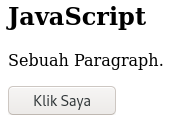
\includegraphics[scale=.7]{1.png} 
    
\includegraphics[scale=.7]{1a.png} 
\end{center}

\subsubsection{Praktik 2}
\textbf{Eksternal JavaScript\\}
\begin{lstlisting}
<!DOCTYPE html>
<html>
    <head>
    </head>
    <body>

        <h2>JavaScript</h2>

        <p id="demo">Sebuah Paragraph.</p>

        <button type="button" onclick="myFunction()">Klik Saya</button>

        <script type="text/javascript" src="eksternal-javascript.js"></script>

    </body>
</html>
\end{lstlisting}
Dokumen html tersebut memiliki script javascript eksternal, sehingga tag elemen script harus menggunakan src, untuk
menunjukkan lokasi file javascript berada. Isi dari file javascript tersebut seperti berikut:
\begin{lstlisting}
function myFunction() {
    document.getElementById("demo").innerHTML = "Paragraph berubah.";
}
\end{lstlisting}
Script tersebut menggunakan fungsi getElementById untuk membaca elemen HTML dengan id demo, kemudian merubah isi dari
elemen html tersebut.
\begin{center}
    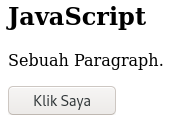
\includegraphics[scale=.7]{1.png} 
    
\includegraphics[scale=.7]{1a.png} 
\end{center}

\subsubsection{Praktik 3}
\textbf{JavaScript document.write\\}
\begin{lstlisting}
<!DOCTYPE html>
<html>
    <body>

        <h1>JavaScript document.write</h1>
        <p>Hasil dari 5 + 6 adalah = </p>

   <script>
       document.write(5 + 6);
   </script>

    </body>
</html>
\end{lstlisting}
Script pada dokumen html tersebut menggunakan document.write, yaitu script untuk menuliskan pada dokumen HTML. Pada hal
ini document.write akan menuliskan hasi operasi penjumlahan 5 dengan 6.
\begin{center}
    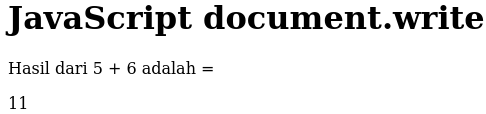
\includegraphics[width=.8\linewidth]{2.png} 
\end{center}

\subsubsection{Praktik 4}
\textbf{JavaScript window.alert\\}
\begin{lstlisting}
<!DOCTYPE html>
<html>
    <body>

        <h1>JavaScript windows.alert</h1>
        <p>Hasil dari 5 + 6 adalah = </p>

   <script>
       window.alert(5 + 6);
   </script>

    </body>
</html>
\end{lstlisting}
Script pada dokumen html tersebut menggunakan window.alert, yaitu script untuk menampilkan jendela pop up. Pada hal
ini window.alert akan menampilkan hasi operasi penjumlahan 5 dengan 6.
\begin{center}
    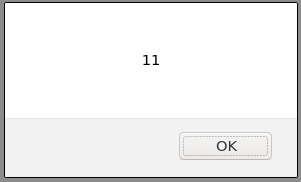
\includegraphics[scale=.7]{3.png} 
\end{center}

\subsubsection{Praktik 5}
\textbf{JavaScript variable dan tipe data\\}
\begin{lstlisting}
<!DOCTYPE html>
<html>
    <body>

        <h2>JavaScript Variabel dan Tipe Data</h2>

        <p> Belajar JavaScript variabel dan tipe data</p>

        <p id="demo"></p>

   <script>
       var x = 5;
       var y = "STMIK AKAKOM";

       document.getElementById("demo").innerHTML =
           "Ini adalah isi dari variabel x dengan tipe data number : " + x +
           "dan ini adalah isi dari variabel y dengan tipe data string : " + y;
   </script>

    </body>
</html>
\end{lstlisting}

Untuk mendeklarasikan variabel pada javascript dapat menggunakan fungsi var, pada javascript di atas javascript akan
mendeklarasikan variabel, lalu menampilkannya.
\begin{center}
    
\includegraphics[width=.8\linewidth]{4.png} 
\end{center}

\subsection{Latihan}
Berikut ini merupakan halaman web yang menampilkan alert yang berisi nama dari halaman
tersebut.
\begin{lstlisting}
<!DOCTYPE html>
<html>
    <head>
        <title>Halaman Latihan 1</title>
    </head>
    <body>

        <h2>Halaman Latihan 1</h2>

       <script>
           window.alert("Anda berada di " + document.title);
       </script>


    </body>
</html>
\end{lstlisting}
Untuk halaman lainnya formatnya sama persis. Untuk menampilkan notifikasi digunakan alert, kemudian untuk mengambil
title dari laman tersebut digunakan document.title.
\begin{center}
    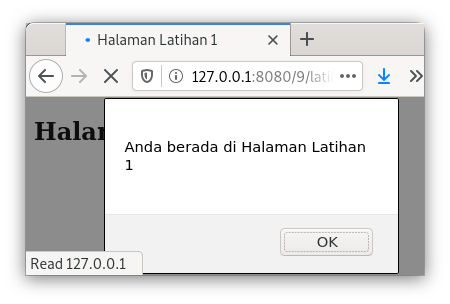
\includegraphics[scale=.4]{5.png} 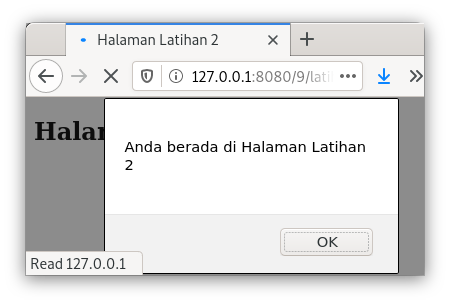
\includegraphics[scale=.4]{5a.png} 
    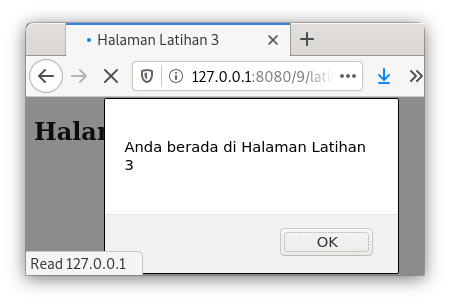
\includegraphics[scale=.4]{5b.png} 
\end{center}

\newpage

\section{Kesimpulan}
Setelah praktik mahasiswa mampu menuliskan script javascript internal dan eksternal, untuk perintah input/output (document.write, prompt, alert), sesuai
aturan penulisan program, menerapkan variabel dan tipe data.

\end{document}
